\documentclass[11pt]{article}
\usepackage[a4paper,margin=22mm]{geometry}
\usepackage{amsmath,amssymb,booktabs,longtable,graphicx,array,xurl}
\usepackage[round,authoryear]{natbib}
\usepackage[colorlinks=true,urlcolor=blue,citecolor=blue,linkcolor=blue]{hyperref}
\usepackage[T1]{fontenc}
\newcommand{\file}[2]{\href{https://github.com/alectionary/vibe-math/blob/master/formalization/higgott-quantum-decoding/#1}{\nolinkurl{#2}}}
\renewcommand{\arraystretch}{1.25}
\setlength{\tabcolsep}{3pt}
\setlength{\emergencystretch}{2em}
\title{Sixfold qubit savings with small Bolza codes:\\a replication of Higgott's quantum coding study}
\date{}
\begin{document}\maketitle
\begin{abstract}
We partly replicated Higgott's small-code result: the Bolza memory uses 16 rather than 96 physical qubits, an exact sixfold saving, while its four-logical-qubit failure probability at physical error probability $p=0.001$ is 0.13822 versus 0.13390 read from the published figure; the planar comparator gives 0.13030 versus 0.12977. We cannot establish identical performance or exact recovery of the original simulations: their shot counts and run configuration were not recovered. Across 32 reconstructed curve points, the largest difference from the figure is 0.01334, inside our exploratory absolute margin of 0.02; 16 differences exceed a simultaneous band based on our simulation uncertainty and vector-extraction bounds alone. At $p=0.001$, Bolza has a slightly higher failure probability than the planar code in both the figure and our reconstruction. The resource advantage survives, but equality of error rates does not follow. This study covers Figure 7.14a and small-code parameters, with additional simulations of the second code size; it does not replicate the entire dissertation.
\end{abstract}
\begin{center}\small
\begin{tabular}{p{.27\linewidth}p{.21\linewidth}p{.20\linewidth}p{.12\linewidth}p{.10\linewidth}}
\toprule Claim & Published & Ours & Same direction? & Verdict\\\midrule
Physical qubits, four logical qubits & Bolza 16; planar 96 & 16; 96; ratio 6 & Yes & Match\\
Block failure at $p=.001$ & Bolza .13390; planar .12977 & .13822; .13030 & Yes & Close\\
Identical performance & Described as identical & Gap .00792; simultaneous half-width .00524 & Bolza higher & Partial\\
Embedded distance, $l=1,2$ & 2; 3 & 2; 3 & Yes & Match\\\bottomrule
\end{tabular}
\end{center}
\noindent\small Published values: \citet[pp.~174,177--178, Table~7.2 and Figure~7.14a]{thesis}; error rates are figure-derived estimates, not printed numerical cells. ``Close'' uses an exploratory 0.02 absolute margin. The half-width uses our Monte Carlo uncertainty with Bonferroni adjustment over 32 comparisons; it excludes unknown original sampling uncertainty.\normalsize

\section{What replicated}
The sixfold resource reduction replicated exactly, while the performance curves replicated approximately. At $p=.001$, our Bolza and planar rates are .13822 and .13030, against .13390 and .12977 in Figure~7.14a. The published ordering is preserved at this point. The question is whether a small hyperbolic memory can protect four logical qubits with substantially fewer physical qubits than four planar honeycomb memories. The answer remains favorable for resources, with a measurable performance difference in our reconstruction.

The selected result is a bounded study within a much larger dissertation. Higgott's thesis was submitted on October 1, 2023; UCL catalogs the doctorate as 2024. Chapter~7 studies hyperbolic Floquet codes, whose two-qubit parity measurements change the represented logical operators over time. We read that chapter, the decoder definitions on pp.~41--56, and Appendix~E. Larger code families, thresholds, the 48-fold saving, real-time decoding speed, and other chapters are outside this replication. The closely related preprint provides the vector figure used in the independent source extraction \citep{construction}.

\begin{figure}[ht]\centering
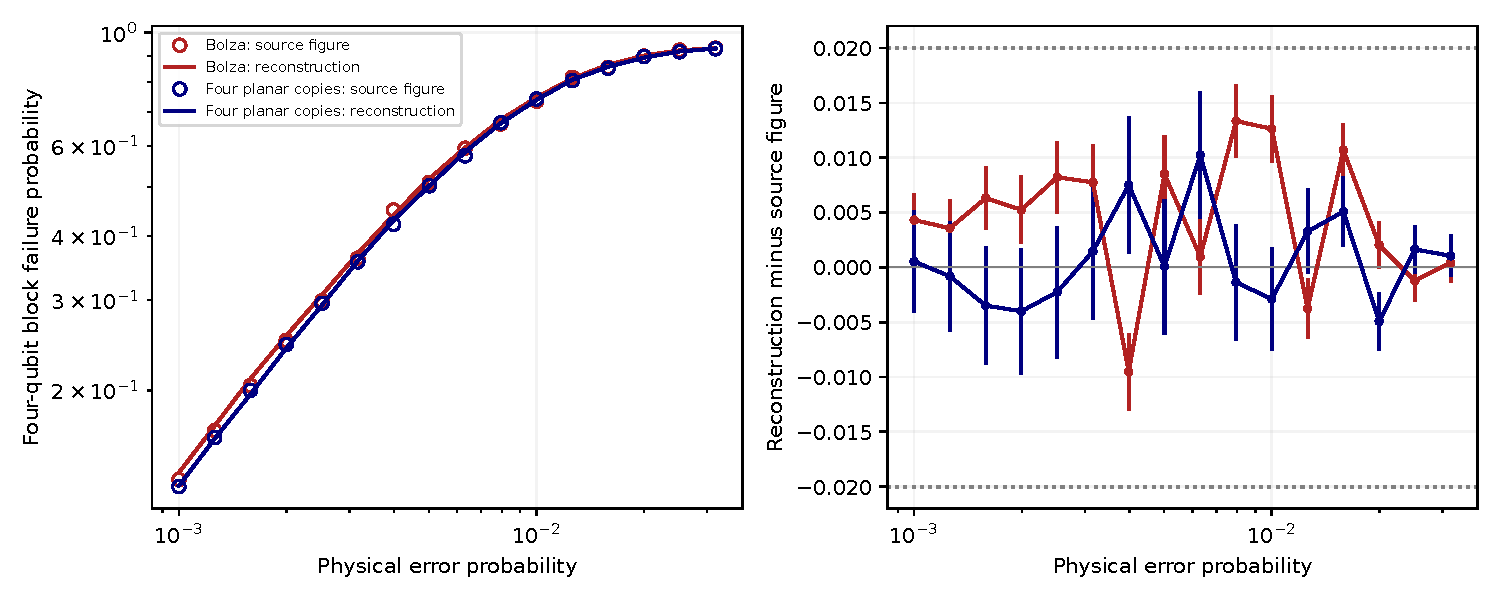
\includegraphics[width=\linewidth]{figure_7_14a_replication.pdf}
\caption{Figure~7.14a reconstructed at 16 physical-noise probabilities. Open circles are independently extracted source-vector coordinates; lines are our 100,000-shot simulations per basis. The right panel gives differences with Bonferroni bands for our sampling uncertainty only. Source sampling uncertainty is unknown. The dotted horizontal lines mark the exploratory 0.02 absolute margin. Data: \file{results/figure_comparison.csv}{figure_comparison.csv}.}
\end{figure}

\section{What we did and what came from the source}
We independently reconstructed noise, checked code parameters, simulated circuits, and compared the resulting curves. The source supplied the Bolza edge schedules, detector definitions, and observable parities as Stim circuit data; the planar geometry and schedules came from the comparator generator cited by the thesis \citep{honeycomb}. We did not independently regenerate the hyperbolic tiling from a group presentation. Our parameter check instead reconstructed the three edge matchings and their faces from the supplied noiseless circuits.

Binary linear algebra verifies that both small lattices have Euler characteristic $-2$ and encode four logical qubits. The 16-qubit lattice has 24 edges and six faces; its 64-qubit refinement has 96 edges and 30 faces. Exhaustive low-weight searches in all three restricted codes recover embedded distances 2 and 3, independently of Stim's circuit-distance routine. For the 64-qubit code, one sector has no logical vector through weight four; the complementary sector has distance three, which suffices to establish the minimum. See \file{code_parameters.py}{code_parameters.py} and \file{provenance/independent_code_parameters.json}{independent_code_parameters.json}.

Stim's graphlike circuit distances independently agree with those embedded minima for reconstructed EM3 circuits. The supplied 16-qubit SD6 circuits also give distance two and use 40 physical qubits. The $l=2$ SD6 total of 160 follows from the source's $n+3n/2$ resource formula, but we have not independently reconstructed its SD6 circuit distance four. That cell is not a numerical replication result.

\section{Methods and uncertainty}
The comparison uses the probability of at least one logical failure, not a mean of four observable error indicators. The thesis defines this convention in Figure~7.11's caption and illustrates independent-patch aggregation in Figure~7.12. If $r_X,r_Z$ are single-patch planar failure probabilities, our four-copy quantity is
\[
 R_{\mathrm{planar}}=\tfrac12\{1-(1-r_X)^4+1-(1-r_Z)^4\}.
\]
For Bolza, each experiment already encodes four logical qubits; we average its X- and Z-basis block probabilities. The four copies are assumed independent, but the four observables within Bolza are not.

We ran 226 conditions with 100,000 shots each, totaling 22.6 million primary and diagnostic shots. This includes both durations, both planar noise variants, both bases, and all planar comparator sizes for the second Bolza code. Seeds, counts, circuit hashes, and processing times are saved for every condition by \file{run_replication.py}{run_replication.py}. Separate historical and generator checks add further samples; these are not silently pooled into the primary estimates.

Our uncertainty calculations separate three sources of error. For an independently sampled basis with empirical rate $r$ and $N$ shots, the estimated variance is $r(1-r)/N$. We propagate the planar transformation with derivative $4(1-r)^3$ and divide the sum of independent basis variances by four when averaging. The two-standard-error bands and Bonferroni bands with multiplier 3.16282 are both saved. The simultaneous construction uses the union bound over 32 comparisons \citep{multiple}. These normal approximations are used for the primary high-count curves, not as precise rare-event confidence bounds for the second code's smallest rates.

Vector-coordinate bounds are not statistical error bars. The independent source reviewer allowed $\pm .05$ original PDF points and propagated that interval through the logarithmic axes. All 32 marker centers were independently aligned to the thesis panel, with maximum residual $1.47\times10^{-5}$ thesis PDF points. Original simulation shot counts were not recovered. Consequently, the 16 conditional band exceedances are differences relative to our precision, not 16 demonstrated failures of the original sampling procedure. A two-sample Monte Carlo test is unavailable.

Our practical comparison margin is explicitly exploratory. We fixed an absolute probability margin of .02 after pilots and before the full curve summary, not in a preregistration and not because the source specified it. Every point estimate lies inside this margin relative to the figure. The largest reconstructed Bolza--planar gap is .01638, but its simultaneous uncertainty can extend to .02347. We therefore do not establish uniform equivalence inside .02 over the entire grid.

\section{Assumptions supplied in this replication}
\subsection{A finite grid and finite sampling budget}
Our numerical scope is the 16 plotted probabilities from .001 to about .03162 for the first size. The second size is a five-point extension at .001, .002, .005, .01, and .02. Each basis uses a fixed 100,000 shots; zero failures, if present, would not imply zero risk. Pilot timings determined feasible batch sizes of 8192 and two worker processes within a four-core quota and 16~GiB memory limit. No hardware-independent speed claim is made.

\subsection{Modern and historical software}
Our primary implementation uses Stim 1.16.0 and PyMatching 2.4.0 because the thesis specifies stabilizer simulation and minimum-weight perfect matching \citep{stim,matching}. A separate Python 3.10 environment uses Stim 1.12.0 and PyMatching 2.1.0, representative of the thesis period, on all 64 primary basis circuits. These are sensitivity versions, not a recovered original environment. Python 3.12.14, NumPy 2.5.4, SciPy 1.18.1, NetworkX 3.7, and Matplotlib 3.11.2 support array calculations, uncertainty, independent graph optimization, and figures \citep{software}. Exact dependencies are in \file{provenance/requirements-lock.txt}{requirements-lock.txt}.

\section{Ambiguities resolved by checks}
\subsection{Measurement duration}
Forty-eight subrounds are the source-consistent duration for Figure~7.14a. Page~157 defines a round as three subrounds, and page~162 describes six subrounds as two rounds. The figure caption says 16 rounds, while the supplied circuit filenames and actual schedules contain 96 subrounds. We reduced the bulk repeat count from 15 to seven, preserving initial and final boundary operations. Both versions were run; the longer circuit substantially raises the low-noise failure probability. The mismatch is an input-selection issue, not evidence that the plotted simulation used the supplied template unchanged. See \file{circuits.py\#L6}{circuits.py}: \texttt{with\_duration}.

\subsection{Correlated EM3 events and a simulation helper}
The EM3 channel requires a correlated event, not independent depolarization and measurement noise. Section~7.2.5.1 samples uniformly from 32 two-qubit Pauli/measurement-flip possibilities with probability $p$, including the identity outcome. A channel with all 31 nonzero binary generators applied independently at probability
\[
 q=\frac{1-(1-p)^{1/16}}2
\]
has the same distribution: every nontrivial character encounters 16 generators, giving $(1-2q)^{16}=1-p$. The implementation is \file{circuits.py\#L19}{circuits.py}: \texttt{em3}. Direct convolution agrees within $7.8\times10^{-16}$. Every one of the 768 event blocks in each supplied EM3 basis circuit contains precisely those 31 generators. Stored $q=.0000312647$ implies $p=.00100000134578$; this rounding is immaterial at our precision. The extra simulation qubit is a noiseless parity-measurement helper, not a seventeenth physical EM3 qubit.

\subsection{Boundary noise in the planar comparator}
The generator's plotting scripts map the displayed label EM3 to its \texttt{EM3\_v3} model. An example collection command uses \texttt{EM3\_v2}; the two models differ at single-qubit boundary measurements. Running both changes the four-copy result at $p=.001$ from .15755 (v2) to .13030 (v3), the latter close to the figure's .12977. We retained all v2 results as a failed reconstruction diagnostic rather than discarding them. This correction follows inspected source code and improves source alignment; it does not constitute fitted calibration of $p$.

\subsection{Non-symplectic observable representatives}
The repository's warning about logical representatives does not by itself invalidate the block-failure statistic. At a common bulk time, the four X sensitivities commute with one another, as do the four Z sensitivities; their cross-commutation matrices have binary rank four for both code sizes. They can therefore be converted into symplectic bases by invertible within-sector transformations. For such a transformation $A$, $e=0$ if and only if $Ae=0$, so the any-failure event is invariant. This argument uses the source's same embedded-code sectors and does not establish equality of individual-observable rates. The matrices are in \file{provenance/logical_basis_audit.json}{logical_basis_audit.json}.

\section{Independent correctness checks}
Independent checks support the implementation, while bounding what they verify. A mutually exclusive categorical representation of the noise was compared with the independent-generator representation on ten code/basis arms with 100,000 shots per generator. The largest standardized difference was 2.962, below a Bonferroni-adjusted threshold for ten two-sided comparisons. All ten noiseless circuits produced zero detector and observable events in 4096 samples each. Exact no-correction probabilities computed from the detector-model characteristic function provide another control, independent of decoding (\file{run_replication.py\#L8}{run_replication.py}: \texttt{no\_correction\_exact}).

A separate NetworkX shortest-path and matching calculation (\file{independent_checks.py\#L26}{independent_checks.py}: \nolinkurl{independent_minimum}) checked 100 syndromes per arm. Its minimum objective differed from PyMatching by at most $1.26\times10^{-6}$ across 1000 cases. This checks optimization on the same graph; it does not independently derive that graph or rule out alternative equal-weight logical corrections. The categorical sampler still uses Stim's stabilizer engine. These are complementary checks, not entirely independent end-to-end implementations. Results and algorithms: \file{independent_checks.py}{independent_checks.py} and \file{provenance/independent_checks.json}{independent_checks.json}.

The external generator's relevant tests pass, but its entire selected suite does not. After one SciPy import-location compatibility change, 270 tests passed and 20 failed; the failures concern SD6/SI1000 decomposed-distance expectations under the modern Stim version. The EM3 subset passes all 122 selected tests. Those unrelated failures remain recorded and were not edited away. The workflow's own 25 tests also pass.

\section{What remains unresolved}
The remaining curve differences cannot yet be assigned to one cause. The largest modern difference from a source point is .01334; the historical-version maximum is .01346, so a broad change in library vintage does not close the gap. At $p=.001$, historical software gives Bolza .13803 and planar .13017, close to the modern values. The duration correction and planar boundary model resolve much larger gaps, but do not recover every source marker.

We rank the remaining causes by available evidence rather than claiming an author error. First, the original run manifest, circuits, graph-conversion choices, seeds, and shot counts are missing; that single run bundle would allow an exact procedural comparison and a legitimate two-sample uncertainty calculation. Second, small boundary or tie-handling differences may survive despite matching code distances and graph objectives. Third, source Monte Carlo fluctuation is plausible but cannot be quantified without counts. The historical graph-import policy was also tested on all 64 primary basis circuits using identical samples for the native and alternative decoders. At $p=.001$, its planar four-copy rate is .10321, farther from the figure than the native .13050 in that paired diagnostic; Bolza changes only from .13749 to .13828. This does not close the source gap. The adapter omits artificial weight-$10^{10}$ dummy edges rejected by modern PyMatching; the diagnostic therefore isolates the graph policy rather than reproducing the entire old decoder unchanged. See \file{provenance/graph_conversion_results.json}{graph_conversion_results.json}. The observed vector-extraction bounds and stored channel rounding are much too small to explain the larger residuals. Numerical optimizers and alternative noise-generation representations agree sufficiently well to make a large implementation fault less plausible.

The second size is supporting evidence, not a complete numerical replication of Figure~7.14b. We ran the reconstructed 64-qubit code and all three planar sizes at five noise strengths and both durations. At $p=.001$ and 48 subrounds, rates are .00209 for Bolza, .13030 for four distance-two patches, .00489 for four distance-three patches, and .00056 for four distance-four patches. The 216/64 ratio is exactly 3.375, but those new simulations do not establish pointwise recovery of the second published panel. Nor do we claim to have reproduced the 64-qubit SD6 distance.

\section{Code and source availability}
The supplied circuit data and comparator source are available locally with their licenses and pinned upstream revisions. The Bolza source revision is \nolinkurl{457975f0d6c67b3a505aacf44589d36779f5dcc1}; the comparator revision is \nolinkurl{cc33baac44c7831bd643db81d0053f8ec6eae9d8}. The latter includes a documented one-line compatibility patch. The separate five-page companion, \nolinkurl{Higgott_Chapter_7_Figure_7_14_Source_Evidence_Appendix.pdf}, supplies six independently reviewed source crops and is delivered alongside this paper. The source dissertation PDF was read through Library after the direct local download returned HTTP~403. Its original bytes, extraction program, and independently prepared 600-dpi source crops are separate source-review inputs, delivered separately from the local simulation bundle.

The dated search ledger distinguishes not recovered from nonexistent. Targeted searches covered the identified GitHub data and comparator repositories, OSF, Zenodo, and GitLab. We did not clone every unrelated repository on the author's account; that workflow departure is recorded. The source reviewer inspected the arXiv v1 archive and found vector figures but no original shot-count arrays. See \file{provenance/availability_and_compliance.json}{availability_and_compliance.json} and \file{source/figure_provenance.json}{figure_provenance.json}.

\section{Next steps}
The original Figure~7.14 run bundle is the most useful next input. With its per-basis counts, exact circuits, software versions, and decoder settings, the residual differences can be separated into sampling fluctuation and procedural differences. Independent vector extraction of Figure~7.14b would extend the second-size comparison, and an independently reconstructed SD6 circuit would test its distance-four cell. Neither missing input is necessary to verify the sixfold integer resource ratio, but both matter for stronger replication claims.

\appendix
\section{Artifacts and reproduction}
The local package contains the runnable inputs, code, outputs, and editable manuscript. The starting master revision \nolinkurl{ca1d06209b03cad666db0a2ffb9678abc89a6b71} records workflow provenance only; it does not contain this new study. The precise local snapshot and commands are documented in \file{README.md}{README.md}. Repository links below are intended master navigation paths; this study has not been published or merged, so new links will not resolve on master until publication.

\begin{longtable}{p{.29\linewidth}p{.62\linewidth}}
\toprule Claim or task & Evidence and regeneration\\\midrule
Resource and embedded distance & \file{code_parameters.py}{code_parameters.py}; run with \texttt{--source inputs/bolza}.\\
Curve simulations & \file{run_replication.py}{run_replication.py}; fixed shots and seed rules in README, ``Rerun simulations.''\\
All source comparisons & \file{results/figure_comparison.csv}{figure_comparison.csv}; regenerate with \file{summarize.py}{summarize.py}.\\
Initial supplied-data pilot & \file{audit_supplied_circuits.py}{audit_supplied_circuits.py}; explicit source and output arguments in README.\\
Independent checks & \file{independent_checks.py}{independent_checks.py}; \file{provenance/independent_checks.json}{independent_checks.json}.\\
Historical version sensitivity & \file{historical_check.py}{historical_check.py}; \file{provenance/historical_results.json}{historical_results.json}.\\
Graph import sensitivity & \file{graph_conversion_check.py}{graph_conversion_check.py}; \file{provenance/graph_conversion_results.json}{graph_conversion_results.json}.\\
Source estimates & \file{source/figure_7_14a_vector_values.csv}{figure_7_14a_vector_values.csv}; supplied source extraction; raw shot arrays absent.\\
Software and compatibility & \file{provenance/requirements-lock.txt}{requirements-lock.txt}; \file{provenance/honeycomb_scipy_compat.patch}{honeycomb_scipy_compat.patch}.\\
Paper rebuild & \file{paper/sixfold_qubit_savings__a_replication_of_higgott_bolza_codes.tex}{sixfold_qubit_savings__a_replication_of_higgott_bolza_codes.tex}; two \texttt{pdflatex} passes from the paper directory.\\\bottomrule
\end{longtable}

\section{Numerical comparisons and reconstruction scope}
Each row compares a source-vector estimate with our calculation. Numerical ``close'' uses the explicitly stated .02 absolute margin; five displayed decimals describe our presentation, not five-decimal precision claimed by the dissertation. Every row has limited reconstruction scope because the original sampling stream and configuration were not obtained. The reason for every ``close'' label is that its absolute difference is below .02. Conditional statistical exceedances remain separately recorded in \file{results/figure_comparison.csv}{figure_comparison.csv}.
\begin{longtable}{llrrrrll}
\toprule Code & $p$ & Source & Ours & Difference & Precision & Numerical & Scope\\\midrule
\endhead
Planar & 0.00100 & 0.12977 & 0.13030 & +0.00053 & 5 d.p. & close & limited \\
Planar & 0.00126 & 0.16177 & 0.16096 & -0.00081 & 5 d.p. & close & limited \\
Planar & 0.00158 & 0.20011 & 0.19663 & -0.00349 & 5 d.p. & close & limited \\
Planar & 0.00200 & 0.24582 & 0.24182 & -0.00400 & 5 d.p. & close & limited \\
Planar & 0.00251 & 0.29586 & 0.29361 & -0.00225 & 5 d.p. & close & limited \\
Planar & 0.00316 & 0.35648 & 0.35795 & +0.00147 & 5 d.p. & close & limited \\
Planar & 0.00398 & 0.42221 & 0.42971 & +0.00751 & 5 d.p. & close & limited \\
Planar & 0.00501 & 0.50187 & 0.50193 & +0.00006 & 5 d.p. & close & limited \\
Planar & 0.00631 & 0.57430 & 0.58454 & +0.01024 & 5 d.p. & close & limited \\
Planar & 0.00794 & 0.66657 & 0.66521 & -0.00136 & 5 d.p. & close & limited \\
Planar & 0.01000 & 0.74158 & 0.73869 & -0.00289 & 5 d.p. & close & limited \\
Planar & 0.01259 & 0.80523 & 0.80851 & +0.00328 & 5 d.p. & close & limited \\
Planar & 0.01585 & 0.85187 & 0.85695 & +0.00508 & 5 d.p. & close & limited \\
Planar & 0.01995 & 0.89816 & 0.89324 & -0.00493 & 5 d.p. & close & limited \\
Planar & 0.02512 & 0.91675 & 0.91838 & +0.00164 & 5 d.p. & close & limited \\
Planar & 0.03162 & 0.92956 & 0.93061 & +0.00105 & 5 d.p. & close & limited \\
Bolza & 0.00100 & 0.13390 & 0.13822 & +0.00432 & 5 d.p. & close & limited \\
Bolza & 0.00126 & 0.16695 & 0.17052 & +0.00357 & 5 d.p. & close & limited \\
Bolza & 0.00158 & 0.20442 & 0.21073 & +0.00631 & 5 d.p. & close & limited \\
Bolza & 0.00200 & 0.25045 & 0.25570 & +0.00525 & 5 d.p. & close & limited \\
Bolza & 0.00251 & 0.29911 & 0.30734 & +0.00822 & 5 d.p. & close & limited \\
Bolza & 0.00316 & 0.36249 & 0.37024 & +0.00775 & 5 d.p. & close & limited \\
Bolza & 0.00398 & 0.45012 & 0.44060 & -0.00952 & 5 d.p. & close & limited \\
Bolza & 0.00501 & 0.50980 & 0.51831 & +0.00851 & 5 d.p. & close & limited \\
Bolza & 0.00631 & 0.59439 & 0.59535 & +0.00096 & 5 d.p. & close & limited \\
Bolza & 0.00794 & 0.66262 & 0.67596 & +0.01334 & 5 d.p. & close & limited \\
Bolza & 0.01000 & 0.73440 & 0.74704 & +0.01264 & 5 d.p. & close & limited \\
Bolza & 0.01259 & 0.81753 & 0.81376 & -0.00377 & 5 d.p. & close & limited \\
Bolza & 0.01585 & 0.85466 & 0.86535 & +0.01070 & 5 d.p. & close & limited \\
Bolza & 0.01995 & 0.89946 & 0.90150 & +0.00204 & 5 d.p. & close & limited \\
Bolza & 0.02512 & 0.92386 & 0.92264 & -0.00122 & 5 d.p. & close & limited \\
Bolza & 0.03162 & 0.93202 & 0.93244 & +0.00042 & 5 d.p. & close & limited \\
\bottomrule
\end{longtable}


\section{Workflow compliance}
The scientific workflow is followed where applicable, with explicit limits. Citation support was checked against the thesis passages, original methodological articles, installed package documentation, and pinned source files; a separate structural citation checker verifies citation keys. SEM engines and fit-index comparability records are not applicable to stabilizer decoding. Proof-assistant formalization is not claimed. Source crops and the extraction program remain separately held review inputs; their absence from the local bundle prevents independent local re-extraction. The narrowed availability search is a justified departure rather than an assertion that no other material exists. Publication was not authorized and has not occurred.

\begin{thebibliography}{99}
\bibitem[Higgott(2024)]{thesis} Higgott, O. (2024). \emph{Practical and Efficient Quantum Error Correction}. Ph.D. dissertation, University College London. Submitted October 1, 2023. \url{https://discovery.ucl.ac.uk/id/eprint/10186408/}.
\bibitem[Higgott and Breuckmann(2023)]{construction} Higgott, O., and Breuckmann, N. P. (2023). Constructions and performance of hyperbolic and semi-hyperbolic Floquet codes. arXiv:2308.03750v1. \url{https://arxiv.org/abs/2308.03750v1}. Source data: \url{https://github.com/oscarhiggott/hyperbolic-floquet-data}.
\bibitem[Gidney et al.(2022)]{honeycomb} Gidney, C., Newman, M., and McEwen, M. (2022). Benchmarking the Planar Honeycomb Code. arXiv:2202.11845v3. \url{https://arxiv.org/abs/2202.11845v3}. Generator: \url{https://github.com/Strilanc/honeycomb-boundaries}.
\bibitem[Gidney(2021)]{stim} Gidney, C. (2021). Stim: a fast stabilizer circuit simulator. \emph{Quantum}, 5, 497. \url{https://doi.org/10.22331/q-2021-07-06-497}. Software versions 1.16.0 and 1.12.0: \url{https://github.com/quantumlib/Stim}.
\bibitem[Higgott(2021)]{matching} Higgott, O. (2021). PyMatching: A Python package for decoding quantum codes with minimum-weight perfect matching. arXiv:2105.13082v2. \url{https://arxiv.org/abs/2105.13082v2}. Software versions 2.4.0 and 2.1.0: \url{https://github.com/oscarhiggott/PyMatching}.
\bibitem[Holm(1979)]{multiple} Holm, S. (1979). A simple sequentially rejective multiple test procedure. \emph{Scandinavian Journal of Statistics}, 6(2), 65--70. \url{https://www.jstor.org/stable/4615733}. We use the conservative single-step Bonferroni bound, not the step-down refinement; bibliographic metadata and abstract were accessible, not the complete original article.
\bibitem[Software projects(2026)]{software} Software projects. Version-specific packages used for implementation: Python 3.12.14 (\url{https://www.python.org/}); NumPy 2.5.4 (\url{https://github.com/numpy/numpy}); SciPy 1.18.1 (\url{https://github.com/scipy/scipy}); NetworkX 3.7 (\url{https://github.com/networkx/networkx}); Matplotlib 3.11.2 (\url{https://github.com/matplotlib/matplotlib}). These packages support numerical arrays, normal quantiles, independent graph matching, and plotting respectively. Pytest 9.2.0 (\url{https://github.com/pytest-dev/pytest}) runs the checks; pdfTeX 1.40.26 (\url{https://www.tug.org/texlive/}) renders the paper. The historical environment uses Python 3.10.22, NumPy 1.24.4, SciPy 1.10.1, NetworkX 2.8.8, and Matplotlib 3.7.3, with its dependency lock included.
\end{thebibliography}
\end{document}
